%\documentclass[a4paper]{article}
%\usepackage[T1]{fontenc}
%\usepackage[utf8]{inputenc}
%\usepackage[italian]{babel}
%\usepackage{amssymb}
%\usepackage{amsmath}
%\usepackage{hyperref}
%\usepackage{amsthm}
%\usepackage{graphicx}
\documentclass[journal, a4paper]{IEEEtran}
\usepackage[italian]{babel}
\usepackage{booktabs}
\usepackage{siunitx}%Questo serve a caricare il pacchetto delle unità di misura del sistema internazionale%
\usepackage[utf8]{inputenc}
\usepackage{graphicx} 
\usepackage{url}
\usepackage{amsmath}


\usepackage{keyval}
\usepackage{xcolor}
\usepackage{caption}
\usepackage{tikz}
\usepackage{circuitikz}
\usepackage{authblk}
%\usepackage{hyperref}

\begin{document}


% Define document title and author
	\title{Tecnologie Digitali - Logbook Week 2}
	\author[1]{Salvatore Bottaro}
		\author[2]{Lorenzo M. Perrone}
		\affil[1]{\texttt{salvo.bottaro@hotmail.it}}
		\affil[2]{\texttt{lorenzo.perrone.lmp@gmail.com}}
	\markboth{Tecnologie Digitali - Di Lieto}{}
	\maketitle
	
\begin{abstract}
	Logbook di laboratorio di Tecnologie Digitali, a.a. 2015/2016. Week 3.
\end{abstract}

\section{Come si può chiamare?}

In un modello ideale di op-amp si presuppne un guadagno a ciclo aperto A (\textit{open loop gain}) infinito. Nei dispositivi reali ovviamente tale parametro è finito e dell'ordine di $10^5 - 10^6$. Il modello di op-amp reale cui si fa riferimento è quello in figura \ref{fig:op-amp-real}.

\begin{figure}[htp]
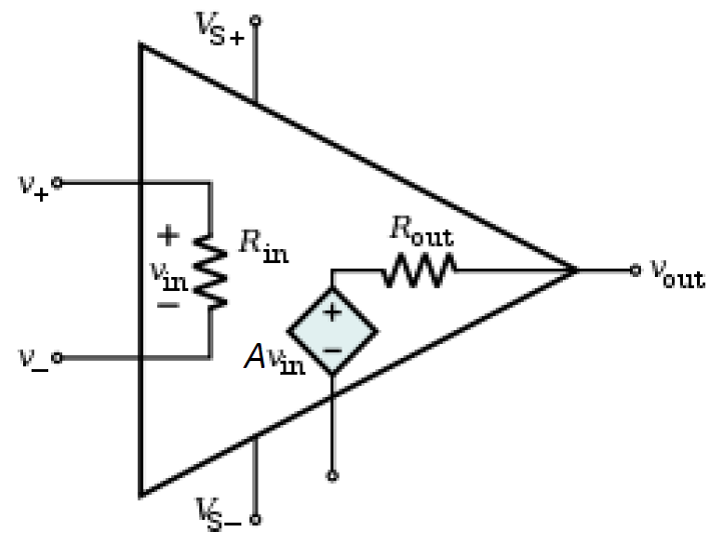
\includegraphics[scale=0.4]{op-amp_real}
\caption{Modello di op-amp reale.}
\label{fig:op-amp-real}
\end{figure}
~\\
$R_{in}$ e $R_{out}$ sono rispettivamente l'impedenza in ingresso e in uscita all'op-amp.
 
\subsection{Hm. 1}
Nel modello ideale si ha $R_{in}$ infinita e $R_{out}$ nulla, mentre per un op-amp reale come il $\mu$A741 il datasheet riporta $R_{in} = 2~ M\Omega$ e $R_{out} = 75 ~\Omega$.\\

Dato che l'open loop gain è finito, si ha che il guadagno in configurazione non-invertente non è più:
\begin{equation}
G_{ideal} = \frac{R_1+R_2}{R_1}
\end{equation}

Ma: 
\begin{equation}
G_{real} = \frac{A}{1+\frac{A}{G_{ideal}}}
\end{equation}

\subsection{Hm. 2}
Rispetto al guadagno ideale si ha, posto $R_1 = 100 ~ \Omega, R_2 = 10~k\Omega, A \approx 10^5$:
\begin{equation}
G_{real}=G_{ideal}~\frac{1}{1+\frac{G_{ideal}}{A}} \approx G_{ideal}~(1-\frac{G_{ideal}}{A}).
\end{equation}
Per cui si ha un errore di circa lo $0.1 \%$ per i valori fissati.

\section{Larghezza di banda}

In figura \ref{fig:tina_par} sono elencati i parametri del modello di op-amp reale di TINA.\\

\begin{figure}[htp]
\centering
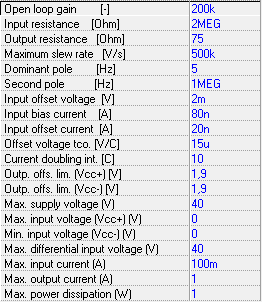
\includegraphics[scale=0.6]{tina_parameters_opamp}
\caption{Elenco dei parametri di TINA per un op-amp $\mu$A741 reale.}
\label{fig:tina_par}
\end{figure}

Si nota come TINA fornisce come valore di open loop gain  A = 200k. I valori delle impedenze in ingresso e in uscita corrispondono con quelli dichiarati nel datasheet. Come input offset voltage, TINA fornisce di default 2 mV che rientra nei limiti 1-6 mV del datasheet. La massima slew rate di TINA corrisponde ai 0.5 $\frac{V}{\mu s}$. I valori della frequenza al primo e al secondo polo sono rispettivamente 5 Hz e 1 MHz; quelli riportati nel datasheet si deducono dal grafico di figura \ref{fig:openloop} e risultano essere circa 4 Hz e 1 MHz.

\begin{figure}[htp]
\centering
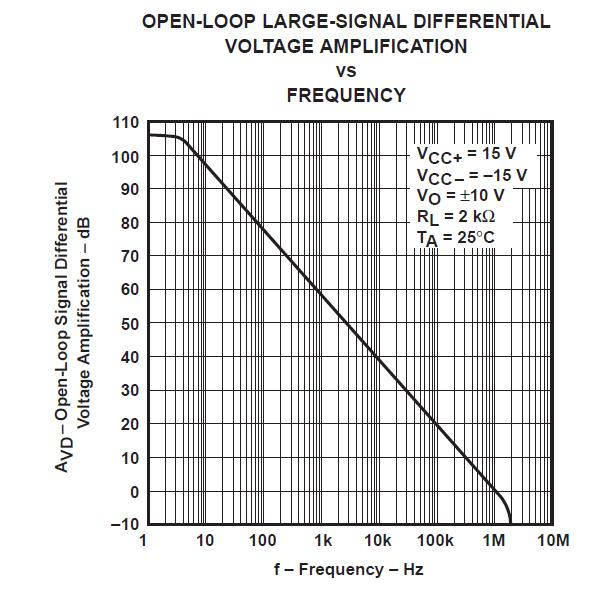
\includegraphics[scale=0.4]{open_loop_gain}
\caption{Grafico dell'open loop gain del $\mu$A741 tratto dal datasheet.}
\label{fig:openloop}
\end{figure}

Abbiamo disegnato con TINA il circuito in figura \ref{fig:tinaes2}.

\begin{figure}[htp]
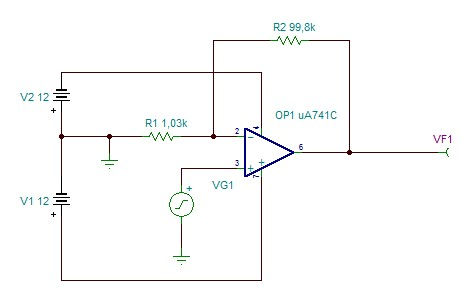
\includegraphics[scale=0.4]{tina_es2}
\caption{Circuito realizzato con TINA. I valori delle resistenze sono quelli impiegati successivamente nel corso dell'esperienza.}
\label{fig:tinaes2}
\end{figure}

Il diagramma di Bode restituito dall' AC transfer characteristic è quello di figura \ref{fig:tina_es2_bode}.

\begin{figure}[htp]
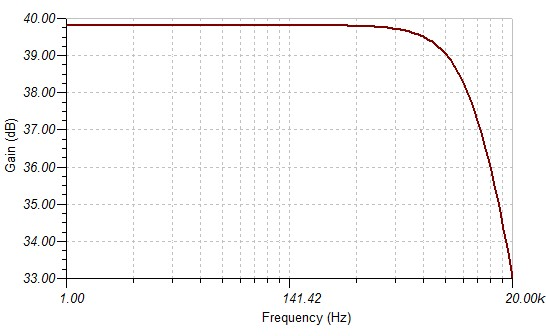
\includegraphics[scale=0.4]{tina_es2_bode}
\caption{Diagramma di Bode del circuito di figura \ref{fig:tinaes2}.}
\label{fig:tina_es2_bode}
\end{figure}

Dalla simulazione si ha che il guadagno a basse frequenza è 39.81 dB, che corrisponde a quello previsto in base alle resistenze scelte. La frequenza di taglio prevista, quella in cui il guadagno scende di 3 dB, è 10.27 kHz, mentre la $f_{\frac{1}{2}}$, quella in cui il guadagno diminuisce di 6 dB, è 17.8 kHz, circa $\sqrt{3}~f_T$, relazione che si riscontra per i filtri passa basso.

\subsection{Hm. 3}
Abbiamo effettuato diverse prove modificando i vari parametri di TINA. Abbiamo riscontrato che la frequenza di taglio dipende in misura maggiore dall' open loop gain e, come è emerso dalla discussione di laboratorio
%Lo, dobbiamo specificarlo secondo te?
, anche dalla frequenza del polo dominante. Dalle prove fatte emerge infatti che vi è proporzionalità diretta fra frequenza di polo dominante e frequenza di taglio e anche fra open loop gain e frequenza di taglio. La frequenza al secondo polo non sembra essere mlto influente poiché variando anche di ordini di grandezza la frequenza al secondo polo, la frequenza di taglio cambia solo di poche centinaia di kHz con dipendenza inversa.

\section{Analisi del generatore ATTEN}

Per verificare le regioni di frequenza, di ampiezza e di offset in cui il generatore fornisce segnali corrtti abbiamo naturalmente effettuato diverse prove variando i precedenti parametri.
Quello che abbiamo riscontrato è che nello spettro di interesse il generatore fornisce segnali puliti finché l'ampiezza picco-picco è più grande di 10-20 mV e l'offset in modulo minore degli 8-9 V. In figura \ref{fig:prova_gen_10khz_100mpp} e \ref{fig:prova_gen_15khz_50mpp} vi sono rappresentati i grafici di segnal "puliti" generati dal generatore.

\begin{figure}[htp]
\centering
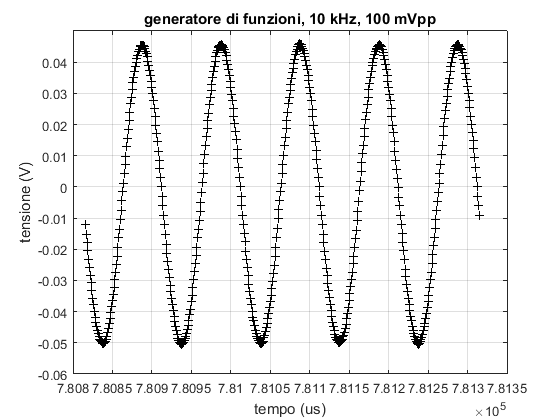
\includegraphics[scale=.4]{prova_gen_10khz_100mpp}
\caption{Segnale a 10 kHz, 100 mV pp e offset nullo.}
\label{fig:prova_gen_10khz_100mpp}
\end{figure}

\begin{figure}[htp]
\centering
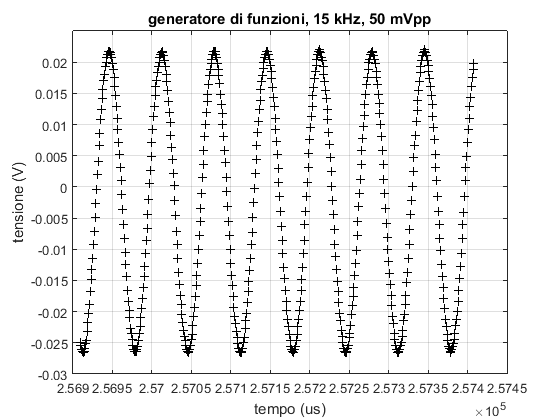
\includegraphics[scale=.4]{prova_gen_15khz_50mpp}
\caption{Segnale a 15 kHz, 50 mV pp e offset nullo.}
\label{fig:prova_gen_15khz_50mpp}
\end{figure}

In figura \ref{fig:prova_gen_10khz_10mpp} e \ref{fig:sballato} si possono osservare invece segnali non perfettamente sinusoidali.

\begin{figure}[htp]
\centering
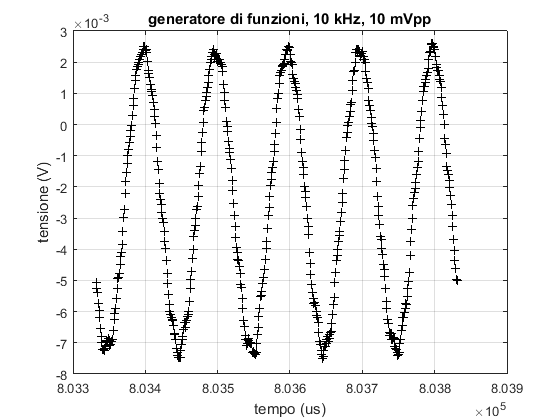
\includegraphics[scale=.4]{prova_gen_10khz_10mpp}
\caption{Segnale a 10 kHz, 10 mV pp.}
\label{fig:prova_gen_10khz_10mpp}
\end{figure}

\begin{figure}[htp]
\centering
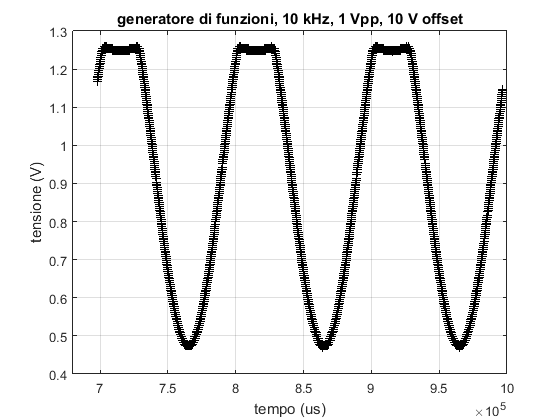
\includegraphics[scale=.4]{sballato}
\caption{Segnale a 10 kHz, 1 V pp e 10 V di offset.}
\label{fig:sballato}
\end{figure}

In particolare in figura \ref{fig:sballato}....
%mi serve il datasheeeeeeeeeeeeeeet!!1!

\section{Analisi in frequenza con il generatore esterno}

Abbiamo collegato il cavo BNC del generatore sia alla CB33 che alla CB68 e avviato l'acquisizione con il VI $BODE_ATTEN$. I dati restituiti a 100k samples al secondo sono mostrati in figura \ref{fig:ampli100000}.

\begin{figure}[htp]
\centering
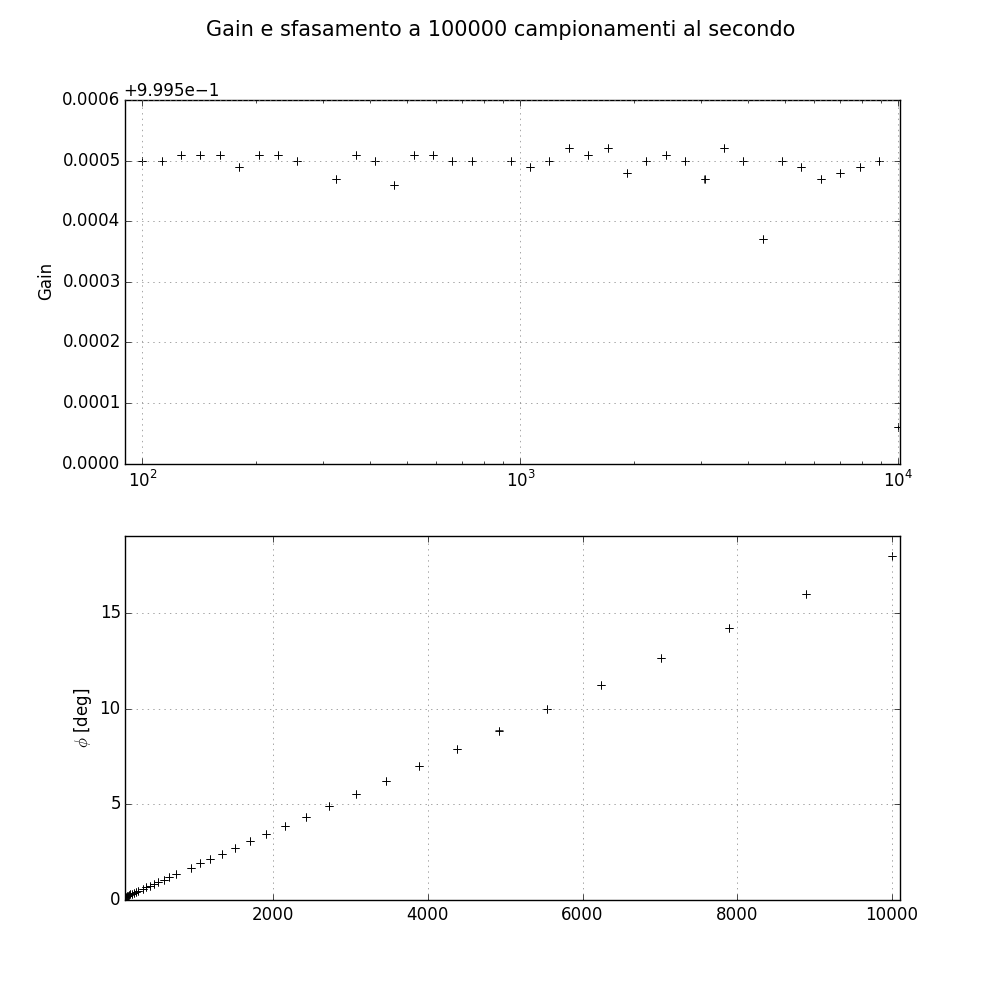
\includegraphics[scale=.3]{subplots_errors_amplitude100000}
\caption{Gain e sfasamento a 100000 campionamenti al secondo.}
\label{fig:ampli100000}
\end{figure}

Come ci si aspettava i punti relativi al guadagno, quindi al rapporto fra le ampiezze del segnale ai due ingressi della DAQ, è compatibile con 1, mentre si osserva un andamento lineare dello sfasamento con la frequenza. Abbiamo ripreso le misure con 200k samples al secondo ottenendo i dati di figura \ref{fig:ampli200000}. 

\begin{figure}[htp]
\centering
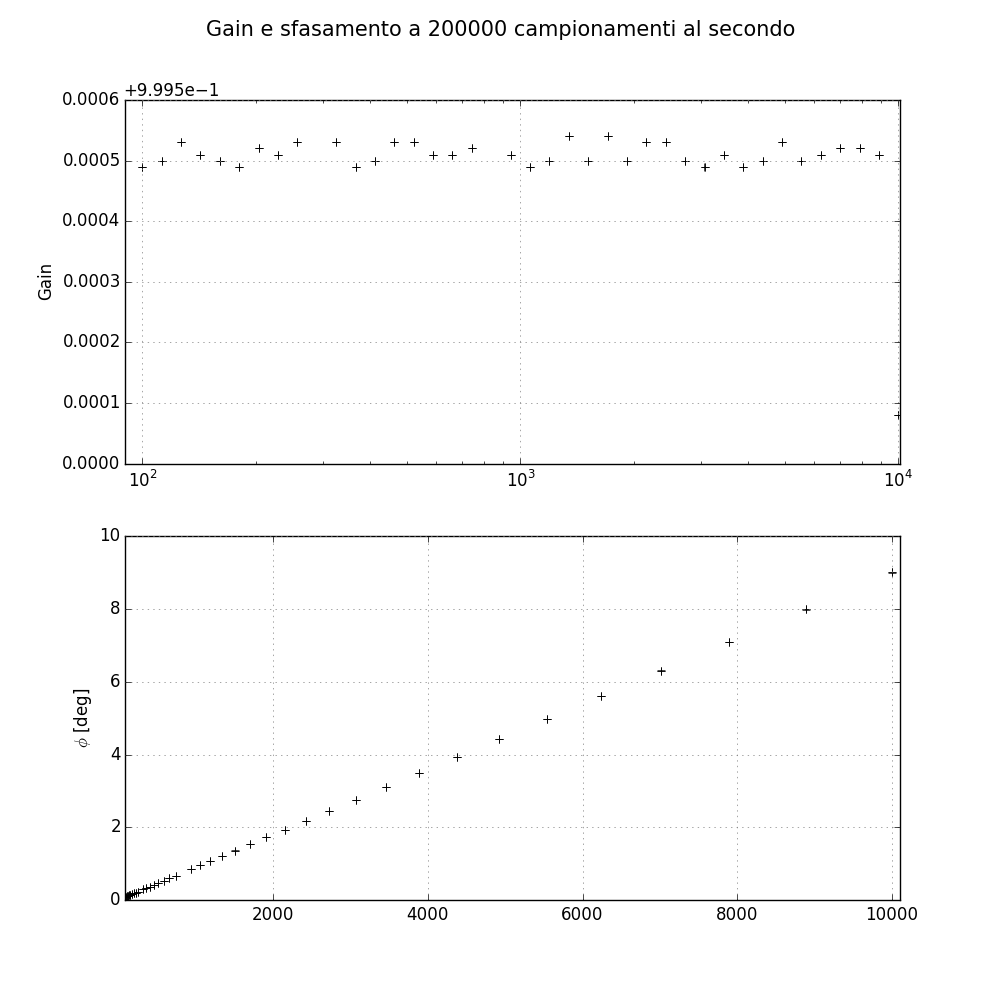
\includegraphics[scale=.3]{subplots_errors_amplitude200000}
\caption{Gain e sfasamento a 200000 campionamenti al secondo.}
\label{fig:ampli200000}
\end{figure}

I dati relativi al gain sono simili al caso precedente mentre per lo sfasamento si osserva ancora un andamento lineare con pendenza dimezzata. Ulteriori prove con frequenze di campionamento superiori presentavano lo stesso andamento sia per il gain che per lo sfasamento.\\
L'osservazione dei dati sperimentali ha suggerito per lo sfasamento una formula del tipo:
\begin{equation}
\Delta \varphi  = \Delta t ~ f
\end{equation}
con:
\begin{equation}
\Delta t = \frac{\alpha}{f_c}
\end{equation}
dove $f_c$ è la frequenza di campionamento. Abbiamo determinato il parametro $\alpha$ tramite fit ottenendo i risultati in tabella \ref{tab:alpha}.
\begin{figure}[htp]
\centering
\caption{Parametro $\alpha$}
\begin{tabular}{|c|c|}
\hline 
$f_c$ & $\alpha$ \\ 
\hline 
100k & 179.97 $\pm$ 0.11 \\ 
\hline 
200k & 179.6 $\pm$ 0.3 \\ 
\hline 
\end{tabular} 
\label{tab:alpha}
\end{figure}

Come si vede i due risultati sono compatibili con 180, per cui $\alpha$ può essere interpretato come parametro di rinormalizzazione in gradi.\\
La ragione di tale comportamento sta nel fatto che i due analog input della scheda non leggono il segnale contemporaneamente, ma come si può leggere dal block diagram del VI prima viene letta la CB68 e dopo un certo intervallo di tempo la CB33, giustificando lo sfasamento proporzionale alla frequenza come è esemplificato in figura \ref{fig:deltat}.

\begin{figure}[htp]
\centering
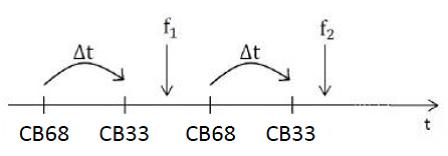
\includegraphics[scale=.55]{deltat}
\caption{Schema esplicativo dell'andamento dello sfasamento in funzione della frequenza}
\label{fig:deltat}
\end{figure}

Per spiegare l'andamento del coefficiente angolare noi abbiamo supposto che all'aumentare della frequenza di campionamento si riducesse il tempo di switch fra le due porte. Di fatti questo è effettivamente corretto nel range di frequenze che abbiamo esplorato noi. In generale però la scheda di acquisizione è programmata per effettuare lo switch fra le due porte sempre nello stesso intervallo di tempo, circa 5 $\mu s$, anche se la frequenza di campionamento è tale che il tempo fra un campionamento e l'altro e più grande di tale intervallo. Tuttavia quando ci si spinge a frequenze di campionamento elevate, la scheda si adatta riducendo il tempo di switch fra le due porte, che è quello che abbiamo osservato noi. Pertanto se ci fossimo spinti a frequenze di campionamento molto basse avremmo dovuto osservare che per frequenze inferiori ad una certa soglia il coefficiente angolare non dipendeva dalla frequenza di campionamento.\\

Per quanto riguarda comunque le frequenze da noi analizzate è possibile fornire un algoritmo correttivo per lo sfasamento che si legge nella seguente espressione:
\begin{equation}
\label{eqn:alg}
\Delta \varphi ' = \Delta \varphi - \alpha ~ \frac{f}{f_c}
\end{equation}
Abbiamo applicato tale algoritmo ai dati precedentemente analizzati ottenendo i grafici in figura \ref{fig:suberr}.

\begin{figure}[htp]
\centering
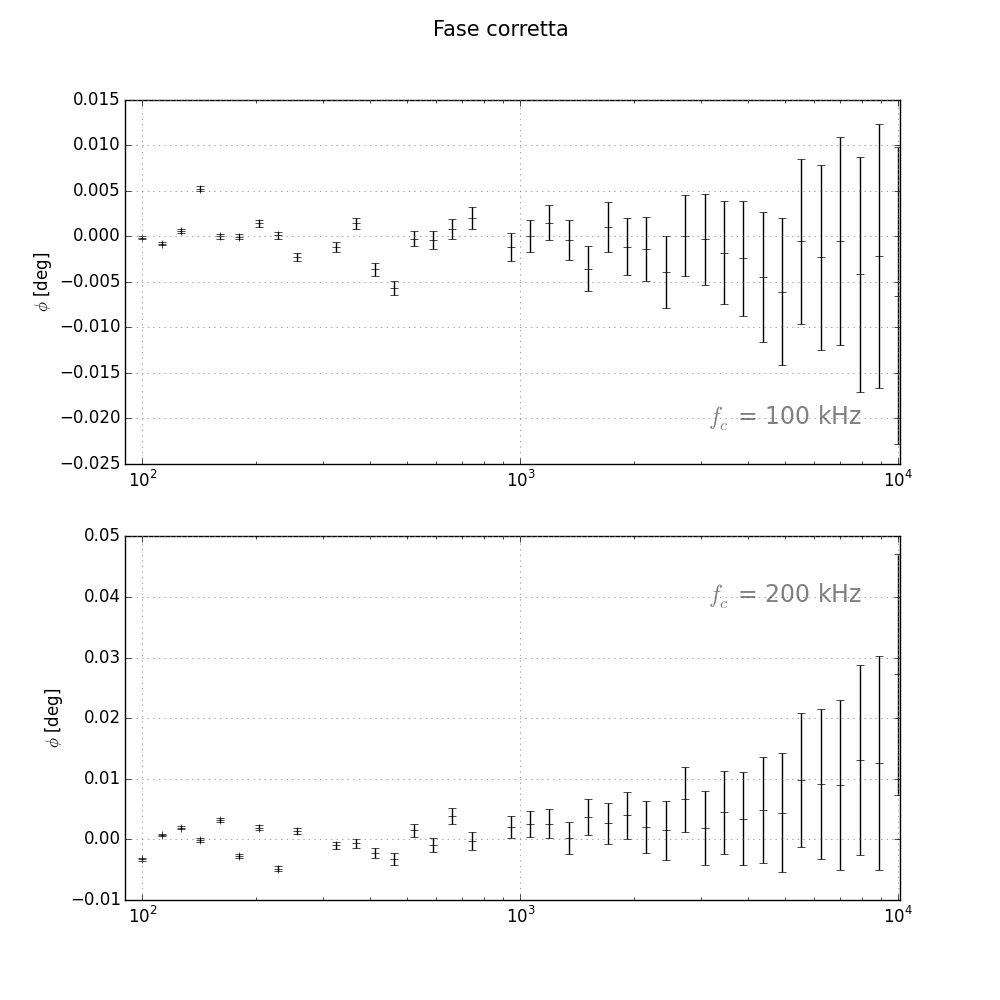
\includegraphics[scale=.3]{subplots_errors}
\caption{Fase corretta tramite l'algoritmo \ref{eqn:alg}}
\label{fig:suberr}
\end{figure}

Gli errori sono stati ottenuti propagando quelli nell'espressione \ref{eqn:alg} e prendendo come errore sulla frequenza $\Delta f = max(5~10^{-5}~f, 40 mHz)$. Il fatto che gli errori aumentassero con la frequenza è stato ritenuto da noi ragionevole perché all'aumentare della frequenza il numero di punti per periodo del segnale diminuisce, il che comporta una maggiore imprecisione nella determinazione della fase. Si noti tuttavia che gli errori rimangono sempre nell'ordine del centesimo di grado. Fittando con rette orizzontali è risultato che per entrambi i grafici le rette fossero compatibili con $ \Delta \varphi =0$.

\section{Analisi in frequenza del circuito con op-amp}

Avendo analizzato a fondo il comportamento del generatore esterno di funzioni, trovando sperimentalmente gli intervalli di frequenza e di tensione in cui aspettarci un buon comportamento ed un segnale piuttosto pulito, abbiamo impostato una frequenza di $230 \si{Hz}$, ed una tensione picco-picco $V_{PP} = 100 \si{mV}$, associati ad un offset \textit{preset} pari a $OFF = -4.60 \si{V}$: si è visto che questo corrisponde ad un offset "effettivo" di $46 \si{mV}$ (l'1\% del valore \textit{preset}), e a queste tensioni è associata un'incertezza di circa $3/4 \si{mV} $. \\
Per queste impostazioni il segnale in uscita non satura il fondoscala da $10 \si{V}$ della nostra \textsc{daq}, e l'offset interno dell'op-amp è compensato il meglio possibile.\\


A questo punto è stato realizzato il circuito in modo tale che il guadagno nominale fosse circa 100, ed è stato tracciato un diagramma di Bode del gain e degli sfasamenti. Si riportano in TABELLA i parametri del circuito con le resistenze scelte e i valori delle grandezze tipiche $f_T, f_{1/2}, G, G \, f_T$. In figura FIGURA è mostrato il diagramma di BODE  del G-100, così come acquisito dal VI.\\

Si noti il confronto con tabella TABELLA dei valori ottenuti tramite la seconda simulazione con TINA, e il notevole accordo con i dati sperimentali.

Introduciamo ora l'algoritmo presentato nella sezione precedente per la correzione degli sfasamenti introdotta dalla routine di acquisizione della scheda DAQ in nostro possesso. L'andamento che ci si aspetta per un circuito amplificante a feedback negativo è mostrato nella figura FIGURA tratta dal manuale 
%\bibitem{M06}
. E' interessante notare come per frequenze anche superiori a $10  f_T$ lo sfasamento non diventi mai maggiore (in modulo) di $-90$, e che in generale, fino alla frequenza del secondo polo, questo non superi mai $180$ (inn modulo) dato che ciò produrrebbe un feedback con interferenza positiva sull'ingresso non invertente \textsc{in+}. In particolare, la differenza fra $180$ e il $\Delta _{f=f2}$, con $f_2$ frequenza di secondo polo, è detta "\textit{phase margin}", ed è un parametro costruttivo dell'integrato.\\

Con l'introduzione dell'algoritmo si può vedere subito che l'andamento degli sfasamenti ricalchi piuttosto fedelmente quello aspettato. Il BODE diagram G-100 "corretto" è mostrato in figura FIGURA, e d'ora in poi le fasi mostrate saranno quelle corrette.\\
 

Continuiamo le acquisizioni tramite il VI \textsc{bode-atten} per verificare il comportamento del nostro op-amp, scegliendo delle resistenze tali da avere un gain di circa 300 e di circa 500. Sono riportate in successione le tabelle con i valori dei parametri dei circuiti e i BODE diagram. Sono d'obbligo due precisazioni:

\begin{itemize}
\item Per il G300, i punti sperimentali mostrati fanno riferimento ad un intervallo delle frequenze $2 \si{kHz} - 20 \si{kHz}$. Questa è la conseguenza del fatto che per ogni configurazione G- sono state effettuate due diverse acquisizioni, la prima in un range molto ampio $100 \si{Hz} - 20 \si{kHz}$, con cui si sono stimate le frequenze caratteristiche, seguita da una seconda acquisizione concentrata nell'intervallo attorno la frequenza di taglio in modo da raffinare la misura. A causa di una nostra sbadatezza per il G-300 la prima serie è stata inavvertitamente cancellata, ma è evidente che i valori riportati nella tabella sono stati misurati propriamente.\\

\item Per ogni configurazione, è stato calcolato il prodotto $ G \, f_T$, che per gli op-amp compensati è una costante costruttiva che identifichiamo con la frequenza del secondo polo, quella a cui, cioè, termina l'andamento costante di $-20 \si{dB} $ per decade, e a cui il gain è unitario (\textsc{UGBW}). I tre valori ottenuti segnalano una tendenza lievemente crescente all'aumentare del gain, pur coincidendo nei limiti dell'errore.
\end{itemize}

Nella tabella seguente sono riportati i valori stimati della frequenza di taglio stimata, tramite il prodotto  $ G \, f_T$, per G1000 e G1. Quest'ultimo valore è ovviamente il \textsc{UGBW} come definito prima. In base al grafico riportato di seguito tratto dal datasheet dell'op-amp %\bibitem{HOP96}
, la frequenza del secondo polo è pari circa a $1 \si{MHz}$, un valore non troppo dissimile da quello da noi ottenuto.

\subsection{Hm. 4}

Abbiamo fatto un'analisi simile a quella di Hm. 2 con il gain 500 dal momento che per il gain 300 non avevamo a disposizione i dati a basse frequenze. In figura \ref{fig:gain500nonsim} si riporta il confronto con i dati sperimentali e la simulazione in cui si è posto 200k come open loop gain. Si può notare come il gain massimo misurato sia significativamente diverso da quello calcolato in base alle resistenze impiegate. Inoltre la frequenza di taglio della simulazione risulta essere 1.95-2.00 kHz mentre quella misurata (1.64 $\pm$ 0.04) kHz.

\begin{figure}[htp]
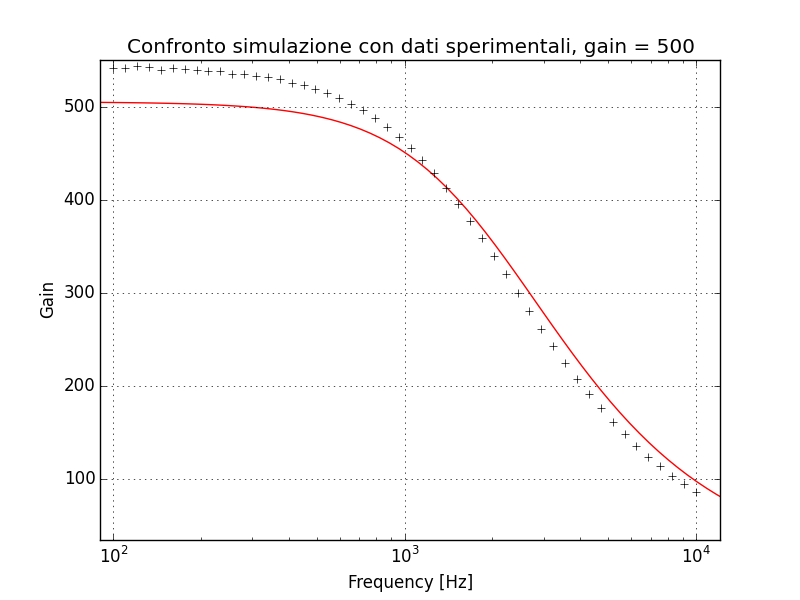
\includegraphics[scale=.4]{hm4comparisons_nonsim}
\caption{Confronto simulazione- dati sperimentali per il gain 500 con 200k di open loop gain.}
\label{fig:gain500nonsim}
\end{figure}

Modificando l'open loop gain dell'op-amp di TINA da 200k a 171k si ottiene il grafico di figura \ref{fig:gain500sim}. Si nota come ancora il gain massimo non corrisponda, però si ha un maggiore accordo ad alte frequenze. Inoltre la fequenza di taglio per questa simulazione vale 1.69 kHz, in perfetto accordo con quella misurata.

\begin{figure}[htp]
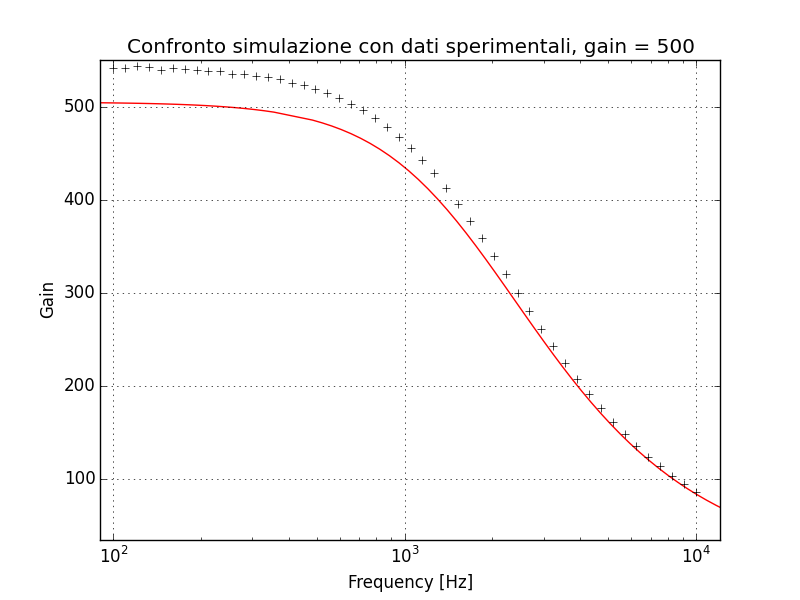
\includegraphics[scale=.4]{hm4comparisons_sim}
\caption{Confronto simulazione- dati sperimentali per il gain 500 con 171k di open loop gain.}
\label{fig:gain500sim}
\end{figure}

\section{Misura della larghezza di banda open-loop}

Questa parte dell'esperienza è volta a misurare il gain open-loop del nostro op-amp, nominalmente di $200k$. Per fare ciò si introduce una resistenza di reazione particolarmente alta, in modo da introdurci il più possibile in regime di assenza di feedback, ottenuto al limite di $R_R \rightarrow \infty $  cioè eliminandola.\\
Ovviamente, per essere capaci di apprezzare gain di quest'ordine, è necessario montare un partitore di tensione resistivo in uscita del generatore esterno, così da non saturare la \textsc{cb68} del DAQ. Purtroppo, per questioni di tempo, e rallentati da alcune acquisizioni completamente saturate, non siamo riusciti a portare a termine questa sezione.



% Now we need a bibliography:
\begin{thebibliography}{5}

	%Each item starts with a \bibitem{reference} command and the details thereafter.
	\bibitem{HOP96} % Transaction paper
	Datasheet, $\mu $A741 General-Purpose Operational Amplifiers. SLOS094E – NOVEMBER 1970  –REVISED JANUARY 2015.
	\url{http://www.ti.com/lit/ds/symlink/ua741.pdf}

	\bibitem{MJ06} % Conference paper
	Product data sheet: 1N4148 High-speed diodes. NXP Semiconductors 2004 Aug 10.
	\url{http://www.nxp.com/documents/data_sheet/1N4148_1N4448.pdf}

	\bibitem{MJH0} % Conference paper
	Product data sheet: AD711 op-amp.
	\url{http://www.analog.com/media/en/technical-documentation/data-sheets/AD711.pdf}
	
	\bibitem{JH06} % Conference paper
	Product data sheet: OP27 op-amp.
	\url{http://www.analog.com/media/en/technical-documentation/data-sheets/OP27.pdf}
	
	\bibitem{JH6} % Conference paper
	Product data sheet: tl081 op-amp.
	\url{http://www.ti.com/lit/ds/symlink/tl081.pdf}

	\bibitem{M06} % Conference paper
	Paul Horowitz, Winfield Hill - The Art of Electronics. Cambridge University Press (1989).
	
\end{thebibliography}

% Your document ends here!
\end{document}